%  LaTeX support: latex@mdpi.com
%  For support, please attach all files needed for compiling as well as the log file, and specify your operating system, LaTeX version, and LaTeX editor.

%=================================================================
% pandoc conditionals added to preserve backwards compatibility with previous versions of rticles

\documentclass[,article,submit,moreauthors,pdftex]{Definitions/mdpi}


%% Some pieces required from the pandoc template
\setlist[itemize]{leftmargin=*,labelsep=5.8mm}
\setlist[enumerate]{leftmargin=*,labelsep=4.9mm}


%--------------------
% Class Options:
%--------------------

%---------
% article
%---------
% The default type of manuscript is "article", but can be replaced by:
% abstract, addendum, article, book, bookreview, briefreport, casereport, comment, commentary, communication, conferenceproceedings, correction, conferencereport, entry, expressionofconcern, extendedabstract, datadescriptor, editorial, essay, erratum, hypothesis, interestingimage, obituary, opinion, projectreport, reply, retraction, review, perspective, protocol, shortnote, studyprotocol, systematicreview, supfile, technicalnote, viewpoint, guidelines, registeredreport, tutorial
% supfile = supplementary materials

%----------
% submit
%----------
% The class option "submit" will be changed to "accept" by the Editorial Office when the paper is accepted. This will only make changes to the frontpage (e.g., the logo of the journal will get visible), the headings, and the copyright information. Also, line numbering will be removed. Journal info and pagination for accepted papers will also be assigned by the Editorial Office.

%------------------
% moreauthors
%------------------
% If there is only one author the class option oneauthor should be used. Otherwise use the class option moreauthors.

%---------
% pdftex
%---------
% The option pdftex is for use with pdfLaTeX. Remove "pdftex" for (1) compiling with LaTeX & dvi2pdf (if eps figures are used) or for (2) compiling with XeLaTeX.

%=================================================================
% MDPI internal commands - do not modify
\firstpage{1}
\makeatletter
\setcounter{page}{\@firstpage}
\makeatother
\pubvolume{1}
\issuenum{1}
\articlenumber{0}
\pubyear{2023}
\copyrightyear{2023}
%\externaleditor{Academic Editor: Firstname Lastname}
\datereceived{ }
\daterevised{ } % Comment out if no revised date
\dateaccepted{ }
\datepublished{ }
%\datecorrected{} % For corrected papers: "Corrected: XXX" date in the original paper.
%\dateretracted{} % For corrected papers: "Retracted: XXX" date in the original paper.
\hreflink{https://doi.org/} % If needed use \linebreak
%\doinum{}
%\pdfoutput=1 % Uncommented for upload to arXiv.org

%=================================================================
% Add packages and commands here. The following packages are loaded in our class file: fontenc, inputenc, calc, indentfirst, fancyhdr, graphicx, epstopdf, lastpage, ifthen, float, amsmath, amssymb, lineno, setspace, enumitem, mathpazo, booktabs, titlesec, etoolbox, tabto, xcolor, colortbl, soul, multirow, microtype, tikz, totcount, changepage, attrib, upgreek, array, tabularx, pbox, ragged2e, tocloft, marginnote, marginfix, enotez, amsthm, natbib, hyperref, cleveref, scrextend, url, geometry, newfloat, caption, draftwatermark, seqsplit
% cleveref: load \crefname definitions after \begin{document}

%=================================================================
% Please use the following mathematics environments: Theorem, Lemma, Corollary, Proposition, Characterization, Property, Problem, Example, ExamplesandDefinitions, Hypothesis, Remark, Definition, Notation, Assumption
%% For proofs, please use the proof environment (the amsthm package is loaded by the MDPI class).

%=================================================================
% Full title of the paper (Capitalized)
\Title{ProyectoTD2025}

% MDPI internal command: Title for citation in the left column
\TitleCitation{ProyectoTD2025}

% Author Orchid ID: enter ID or remove command
%\newcommand{\orcidauthorA}{0000-0000-0000-000X} % Add \orcidA{} behind the author's name
%\newcommand{\orcidauthorB}{0000-0000-0000-000X} % Add \orcidB{} behind the author's name


% Authors, for the paper (add full first names)
\Author{Mar Alemany$^{}$, Martín González$^{}$, Mateo Reina$^{}$, Adrian
Mena$^{}$, Sina Taheri$^{}$}


%\longauthorlist{yes}


% MDPI internal command: Authors, for metadata in PDF
\AuthorNames{Mar Alemany, Martín González, Mateo Reina, Adrian
Mena, Sina Taheri}

% MDPI internal command: Authors, for citation in the left column

% Affiliations / Addresses (Add [1] after \address if there is only one affiliation.)
\address{%
}

% Contact information of the corresponding author
\corres{Correspondence: }

% Current address and/or shared authorship








% The commands \thirdnote{} till \eighthnote{} are available for further notes

% Simple summary

%\conference{} % An extended version of a conference paper

% Abstract (Do not insert blank lines, i.e. \\)


% Keywords

% The fields PACS, MSC, and JEL may be left empty or commented out if not applicable
%\PACS{J0101}
%\MSC{}
%\JEL{}

%%%%%%%%%%%%%%%%%%%%%%%%%%%%%%%%%%%%%%%%%%
% Only for the journal Diversity
%\LSID{\url{http://}}

%%%%%%%%%%%%%%%%%%%%%%%%%%%%%%%%%%%%%%%%%%
% Only for the journal Applied Sciences

%%%%%%%%%%%%%%%%%%%%%%%%%%%%%%%%%%%%%%%%%%

%%%%%%%%%%%%%%%%%%%%%%%%%%%%%%%%%%%%%%%%%%
% Only for the journal Data



%%%%%%%%%%%%%%%%%%%%%%%%%%%%%%%%%%%%%%%%%%
% Only for the journal Toxins


%%%%%%%%%%%%%%%%%%%%%%%%%%%%%%%%%%%%%%%%%%
% Only for the journal Encyclopedia


%%%%%%%%%%%%%%%%%%%%%%%%%%%%%%%%%%%%%%%%%%
% Only for the journal Advances in Respiratory Medicine
%\addhighlights{yes}
%\renewcommand{\addhighlights}{%

%\noindent This is an obligatory section in “Advances in Respiratory Medicine”, whose goal is to increase the discoverability and readability of the article via search engines and other scholars. Highlights should not be a copy of the abstract, but a simple text allowing the reader to quickly and simplified find out what the article is about and what can be cited from it. Each of these parts should be devoted up to 2~bullet points.\vspace{3pt}\\
%\textbf{What are the main findings?}
% \begin{itemize}[labelsep=2.5mm,topsep=-3pt]
% \item First bullet.
% \item Second bullet.
% \end{itemize}\vspace{3pt}
%\textbf{What is the implication of the main finding?}
% \begin{itemize}[labelsep=2.5mm,topsep=-3pt]
% \item First bullet.
% \item Second bullet.
% \end{itemize}
%}


%%%%%%%%%%%%%%%%%%%%%%%%%%%%%%%%%%%%%%%%%%


% tightlist command for lists without linebreak
\providecommand{\tightlist}{%
  \setlength{\itemsep}{0pt}\setlength{\parskip}{0pt}}

% From pandoc table feature
\usepackage{longtable,booktabs,array}
\usepackage{calc} % for calculating minipage widths
% Correct order of tables after \paragraph or \subparagraph
\usepackage{etoolbox}
\makeatletter
\patchcmd\longtable{\par}{\if@noskipsec\mbox{}\fi\par}{}{}
\makeatother
% Allow footnotes in longtable head/foot
\IfFileExists{footnotehyper.sty}{\usepackage{footnotehyper}}{\usepackage{footnote}}
\makesavenoteenv{longtable}


\usepackage{booktabs}
\usepackage{longtable}

\begin{document}



%%%%%%%%%%%%%%%%%%%%%%%%%%%%%%%%%%%%%%%%%%

\hypertarget{introducciuxf3n}{%
\section{Introducción}\label{introducciuxf3n}}

En la actualidad, la digitalización de los tickets de compra se ha
convertido en una práctica común en grandes cadenas de supermercados.
Estos tickets electrónicos, enviados en formato PDF al correo del
cliente, no solo reducen el uso de papel, sino que también generan datos
valiosos que pueden ser analizados para obtener información relevante
sobre los hábitos de consumo, la evolución de precios y las preferencias
de los compradores.

Este proyecto tiene como objetivo desarrollar un sistema de análisis
automatizado que permita extraer, procesar y visualizar la información
contenida en los tickets de Mercadona. Mediante técnicas de tratamiento
de datos en R, exploraremos patrones de compra, identificaremos los
productos más vendidos, analizaremos la evolución temporal de los
precios y determinaremos tendencias en función de la ubicación de la
tienda y el momento de la compra.

\hypertarget{material-y-muxe9todos}{%
\section{Material y Métodos}\label{material-y-muxe9todos}}

Para llevar a cabo este proyecto se han seleccionando un conjunto de
librerías específicas que respondieran a los distintos requerimientos
del análisis.

Para la manipulación de datos se emplearon los paquetes tidyverse
(incluyendo dplyr y stringr), que permitieron realizar operaciones de
filtrado, transformación y procesamiento de texto de manera eficiente.
La extracción del contenido textual desde los archivos PDF se realizó
mediante el paquete pdftools, capaz de preservar la estructura original
de los documentos.

Las visualizaciones se generaron utilizando ggplot2, seleccionado por su
versatilidad para crear gráficos de alta calidad. Para la presentación
de resultados en formatos reproducibles se implementó knitr, facilitando
la integración de código, resultados y texto explicativo.

Utilizaremos dos data frames para manejar los datos de manera más
eficiente. El primer data frame contendrá la información general del
ticket, como la dirección del supermercado, la fecha y hora de la
compra, el monto total, entre otros. En este caso, todos los productos
registrados en el ticket se almacenarán como una sola cadena de texto en
una única variable. El segundo data frame desglosará los productos en
variables separadas

Ambos data frames estarán vinculados a través de la variable fs (factura
simplificada).

\hypertarget{importaciuxf3n-de-los-datos}{%
\section{Importación de los datos}\label{importaciuxf3n-de-los-datos}}

\hypertarget{carga-de-ficheros}{%
\subsection{Carga de ficheros}\label{carga-de-ficheros}}

Para evitar errores durante el procesamiento posterior, se realizó un
cambio en los nombres de los archivos PDF originales. Los archivos
fueron renombrados de forma secuencial con un formato estándar. Esta
acción se llevó a cabo una única vez, y por ello el código
correspondiente fue comentado en el script, con el fin de prevenir que
los archivos se sobrescriban accidentalmente al ejecutar el programa más
de una vez.

Se procedió a cargar automáticamente todos los archivos PDF contenidos
en la carpeta de trabajo designada. Para ello, se empleó una función que
permite listar únicamente los archivos con extensión .pdf, garantizando
así que solo se consideren los documentos relevantes para el análisis.
Esta carga automatizada facilita el procesamiento por lotes y evita la
necesidad de seleccionar manualmente cada archivo.

Para el proyecto se han importado un total de 303 archivos.

\hypertarget{carga-de-datos}{%
\subsection{Carga de datos}\label{carga-de-datos}}

Se construyó un data frame a partir de los datos extraídos, realizando
las transformaciones necesarias para asegurar que cada variable tuviera
el formato y tipo de dato adecuados.

Para la lectura de los archivos PDF se utilizaron funciones de la
librería pdftools, mientras que la limpieza y manipulación de las
cadenas de texto se llevó a cabo con funciones de la librería stringr.

Durante el procesamiento, se asignó el tipo de dato Date a la variable
de fecha y se convirtieron en valores numéricos las variables decimales
como el total de la compra, la base imponible y la cuota de IVA. Cabe
señalar que muchos de los datos no pueden incorporarse directamente al
data frame, ya que en el formato original aparecen combinados en una
misma línea. Es el caso de la fecha, la hora y el número de operación,
que debieron separarse y asignarse a variables distintas.

\begin{table}

\caption{\label{tab:tabla_variables}Descripción de variables}
\centering
\begin{tabular}[t]{cc}
\toprule
Variable & Descripción\\
\midrule
comercio & Nombre del comercio\\
empresa & Tipo y código de empresa\\
direccion & Dirección del comercio\\
cp & Código postal\\
telefono & Teléfono del comercio\\
\addlinespace
fecha & Fecha de la compra (día-mes-año)\\
hora & Hora de la compra (horas y minutos)\\
op & Número del código de la operación\\
fs & Código de la factura simplificada\\
productos & Lista con los productos comprados\\
\addlinespace
total & Dinero total de la compra\\
forma\_pago & Forma de pago (tarjeta o en efectivo)\\
base\_imp & Base imponible (IVA)\\
cuota & Cuota del IVA\\
\bottomrule
\end{tabular}
\end{table}

Las variables finales obtenidas se pueden observar en la Tabla
\ref{tab:tabla_variables}.

Por razones de espacio y legibilidad, no se muestra en el documento el
conjunto de datos (df), ya que contiene un número elevado de
observaciones y variables.

\hypertarget{analizamos-los-productos}{%
\section{Analizamos los productos}\label{analizamos-los-productos}}

La información relativa a los productos comprados se encontraba
inicialmente agrupada dentro de una única columna del data frame
principal. Para facilitar su análisis, se extrajo esta columna a un
nuevo data frame, separando los productos que venían concatenados en una
misma celda.

\hypertarget{productos-pescateria}{%
\subsection{Productos pescateria}\label{productos-pescateria}}

El procesamiento de los productos se realizó en varias etapas, según el
tipo de producto y la forma en que aparecían en el ticket. En primer
lugar, se identificaron los productos de pescadería, que siguen un
formato particular: aparecen siempre precedidos por una línea con la
palabra ``PESCADO'', seguida del nombre del producto en la línea
siguiente y de los detalles de compra (peso, precio por kilo y total) en
una tercera línea. A partir de esta estructura, se extrajeron los datos
relevantes y se almacenaron en un nuevo data frame específico para
pescado.

\begin{table}

\caption{\label{tab:tabla_pescado}Datos procesados para productos de pescadería}
\centering
\begin{tabular}[t]{ccccc}
\toprule
num\_ticket & nombre & peso\_kg & precio\_kg & importe\\
\midrule
168515 & SARDINA GR 13/20 & 0.390 & 6.95 & 2.71\\
433003 & BOQUERÓN MED 51/80 & 0.756 & 4.95 & 3.74\\
075372 & LENGUADO FRESC EUROP & 0.262 & 24.95 & 6.54\\
491735 & CORVINA & 1.560 & 9.95 & 15.52\\
491735 & CIGALA PEQUEÑA REF & 0.222 & 16.85 & 3.74\\
\addlinespace
087622 & LENGUADO FRESC EUROP & 0.376 & 18.95 & 7.13\\
516718 & LENGUADO FRESC EUROP & 0.610 & 18.95 & 11.56\\
696429 & BACALADILLA & 1.590 & 3.95 & 6.28\\
682028 & SARDINA MED 21/35 & 0.366 & 5.95 & 2.18\\
696429 & BACALADILLA & 1.590 & 3.95 & 6.28\\
\bottomrule
\end{tabular}
\end{table}

En la siguiente tabla \ref{tab:tabla_pescado} se pueden observar los
datos procesados para los productos de pescadería .

\hypertarget{productos-vendidos-por-peso}{%
\subsection{Productos vendidos por
peso}\label{productos-vendidos-por-peso}}

Después, se eliminaron las filas correspondientes a productos de
pescadería para poder trabajar exclusivamente con los productos que
también se venden por peso, como frutas y verduras. Estos artículos
generalmente constan de dos líneas: la primera contiene el nombre del
producto y la segunda incluye el peso, el precio por kilogramo y el
importe total. A partir de esta estructura se construyó un segundo data
frame con las frutas y verduras, extrayendo y transformando la
información necesaria.

\begin{table}

\caption{\label{tab:tabla_fruta_verdura}Descripción de variables del conjunto de frutas y verduras}
\centering
\begin{tabular}[t]{ccccc}
\toprule
num\_ticket & nombre & peso\_kg & precio\_kg & importe\\
\midrule
301952 & MANZANA GOLDEN & 1.694 & 1.49 & 2.52\\
168515 & LANGOSTINO COCIDO & 0.424 & 10.95 & 4.64\\
405598 & PATATA & 1.378 & 1.99 & 2.74\\
407209 & PLATANO & 1.202 & 2.75 & 3.31\\
070987 & PATATA & 1.930 & 1.99 & 3.84\\
\addlinespace
070987 & TOMATE ENSALADA & 1.412 & 1.75 & 2.47\\
330410 & PEPINO & 0.652 & 1.45 & 0.95\\
330410 & BANANA & 0.936 & 1.45 & 1.36\\
330410 & PARAGUAYO & 0.594 & 3.79 & 2.25\\
330410 & MANZANA GOLDEN & 1.216 & 2.09 & 2.54\\
\bottomrule
\end{tabular}
\end{table}

En la siguiente tabla \ref{tab:tabla_fruta_verdura} se pueden observar
los datos procesados para los productos de fruta y verdura .

\hypertarget{productos-vendidos-por-unidad}{%
\subsection{Productos vendidos por
unidad}\label{productos-vendidos-por-unidad}}

Una vez separados los productos por peso, se procedió a procesar el
resto de productos, es decir, aquellos que se venden por unidades. En
este caso, se extrajeron datos como la cantidad, el nombre del producto,
el precio unitario y el importe total. Se aplicaron técnicas de
procesamiento de texto para limpiar y estructurar la información, ya que
algunos productos con una sola unidad incluían el precio directamente
dentro del nombre del producto.

\begin{table}

\caption{\label{tab:tabla_productos_unidad}Descripción de variables del conjunto de productos por unidad}
\centering
\begin{tabular}[t]{ccccc}
\toprule
num\_ticket & nombre & cantidad & precio\_unitario & importe\\
\midrule
520925 & DONACIÓN & 5 & 1.00 & 5.00\\
520925 & BARREÑO & 1 & 2.20 & 2.20\\
520925 & PALO ANTIDESLIZANTE & 3 & 1.90 & 5.70\\
520925 & MULTIUSOS & 1 & 2.55 & 2.55\\
520925 & AGUA MINERAL & 2 & 0.73 & 1.46\\
\addlinespace
520925 & B.BASURA EXT.C.FÁCIL & 2 & 1.60 & 3.20\\
520925 & ESCURRE FÁCIL & 1 & 2.85 & 2.85\\
520925 & CUBO FREGAR C/RUEDAS & 1 & 3.85 & 3.85\\
520925 & FRIEGASUELOS PINO & 1 & 0.95 & 0.95\\
520925 & FIBRAS CRUZADAS & 2 & 2.10 & 4.20\\
\bottomrule
\end{tabular}
\end{table}

En la siguiente tabla \ref{tab:tabla_productos_unidad} se pueden
observar los datos procesados para los productos por unidad .

\hypertarget{conjunto-completo-de-productos}{%
\subsection{Conjunto completo de
productos}\label{conjunto-completo-de-productos}}

Finalmente, los tres grupos de productos ---pescado, frutas y verduras,
y productos por unidades--- se combinaron en un único data frame
unificado. A este conjunto se le añadió una columna adicional que
indicaba si el ticket incluía un servicio de aparcamiento, en caso de
que esa información estuviera disponible. El resultado fue un data frame
final, estructurado y homogéneo, con todos los productos organizados por
tipo, cantidad, precio, importe y número de ticket, listo para su
análisis posterior.

\begin{table}

\caption{\label{tab:tabla_final}Descripción de variables del conjunto de datos final}
\centering
\begin{tabular}[t]{ccccccc}
\toprule
num\_ticket & nombre & cantidad & precio & importe & tipo & tiene\_aparcamiento\\
\midrule
007267 & PERA CONFERENCIA & 0.854 & 2.55 & 2.18 & fruta\_verdura & NA\\
007267 & MANZ. ROJA DULCE & 1.474 & 2.90 & 4.27 & fruta\_verdura & NA\\
007267 & PIZZA BOLOÑESA & 1.000 & 2.60 & 2.60 & unidades & NA\\
007267 & MIX FRUTOS ROJOS & 1.000 & 1.66 & 1.66 & unidades & NA\\
007267 & PISTO DE VERDURAS & 1.000 & 2.30 & 2.30 & unidades & NA\\
\addlinespace
007267 & FILETE DE TRUCHA & 1.000 & 3.92 & 3.92 & unidades & NA\\
007267 & PAN SEMILLAS & 1.000 & 1.60 & 1.60 & unidades & NA\\
007267 & SNACK PIPAS & 1.000 & 1.40 & 1.40 & unidades & NA\\
007267 & +PROT NATILLA VAINI & 1.000 & 1.75 & 1.75 & unidades & NA\\
007267 & SNACK CHOCOLATE & 1.000 & 1.50 & 1.50 & unidades & NA\\
\bottomrule
\end{tabular}
\end{table}

En la siguiente tabla \ref{tab:tabla_final} se pueden observar los datos
procesados para los productos por unidad .

\hypertarget{analisis-exploratorio}{%
\section{Analisis exploratorio}\label{analisis-exploratorio}}

\hypertarget{datos-faltantes}{%
\subsection{Datos faltantes}\label{datos-faltantes}}

Realizamos una comprobación para asegurarnos de que el data frame no
contenga valores faltantes (exceptuando la variable aparcamiento, ya que
cuando no se encuentra disponible, se asigna un valor NA). En caso de
encontrar valores faltantes en otras variables, eliminamos las filas
correspondientes.

\hypertarget{anuxe1lisis-univariante}{%
\subsection{Análisis univariante}\label{anuxe1lisis-univariante}}

Comenzaremos el análisis de las variables dividiéndolas en dos grupos:
las variables categóricas y las variables numéricas.

\hypertarget{variables-categuxf3ricas}{%
\subsubsection{Variables categóricas}\label{variables-categuxf3ricas}}

Las variables categóricas representan cualidades o características, y en
nuestro data frame están codificadas como tipo character.

En el data frame de los tickets, la mayoría de las variables son de tipo
categórico. Una de las más relevantes es la variable num\_ticket, que es
única para cada ticket y sirve como identificador.

Otras variables categóricas en nuestro análisis incluyen comercio y
empresa, que son constantes en todos los tickets. Sin embargo, esta
estructura está pensada por si en el futuro se incluyen tickets de otros
comercios o empresas. De manera similar, tenemos la variable
forma\_pago, que actualmente solo contiene registros de pagos realizados
con tarjeta, pero se mantiene por si en algún ticket hay pagos en
efectivo.

En cuanto a las variables categóricas en el data frame de productos,
tenemos tipo, que clasifica los productos en categorías como
``pescado'', ``fruta\_verdura'' y ``unidades''. Además, la variable
nombre contiene los nombres de los productos.

En total, tenemos 0 valores únicos en comercio, 0 valores únicos en
empresa, y 0 valores únicos en forma\_pago.

También observamos que tenemos 3 tipos diferentes de productos y 1396
productos distintos registrados en total.

\hypertarget{variables-de-tipo-numuxe9rico}{%
\subsubsection{Variables de tipo
numérico}\label{variables-de-tipo-numuxe9rico}}

as variables numéricas representan cantidades o medidas cuantitativas
dentro del conjunto de datos. En nuestro análisis, nos centramos
principalmente en dos variables clave: cantidad (ya sea en unidades o en
kilos) y precio (precio por kilo o unitario, según el tipo de producto).

Para tener una visión general del comportamiento de las compras, primero
calculamos el valor total gastado, sumando el importe de todos los
productos. Además, analizamos cuántos productos se compran por ticket
(es decir, la media de la suma de cantidades por cada ticket) y cuál es
el gasto medio por ticket.

El gasto total en todos los productos es: 14022.5 € La media de
productos comprados por ticket es: 19.9 La media del importe total por
ticket es: 48.35 €

Además, observamos que la variable cantidad contiene valores decimales
en algunos casos, lo que se debe a que ciertos productos (como frutas,
verduras o pescado) se venden al peso, mientras que otros se venden por
unidades enteras.

A continuación, mostramos un resumen de las cantidades redondeadas para
tener una idea de las frecuencias de compra por tipo de producto:

\begin{longtable}[]{@{}lr@{}}
\caption{Frecuencia de Cantidades Redondeadas de Productos
Comprados}\tabularnewline
\toprule\noalign{}
Cantidad Redondeada & Frecuencia \\
\midrule\noalign{}
\endfirsthead
\toprule\noalign{}
Cantidad Redondeada & Frecuencia \\
\midrule\noalign{}
\endhead
\bottomrule\noalign{}
\endlastfoot
0 & 79 \\
1 & 4443 \\
2 & 453 \\
3 & 72 \\
4 & 30 \\
5 & 10 \\
6 & 2 \\
7 & 1 \\
8 & 2 \\
\end{longtable}

Con esto, podemos observar que en la mayoría de los casos se compraron 1
o 2 unidades/kilos, siendo 1 la cantidad más frecuente.

\hypertarget{anuxe1lisis-multivariable}{%
\subsection{Análisis multivariable}\label{anuxe1lisis-multivariable}}

\textbf{Relación entre la Dirección y las Ganancias} En este apartado
analizamos si existe alguna relación entre la localización del
supermercado (variable dirección) y los ingresos obtenidos. Para ello,
generamos dos gráficos: uno que muestra la ganancia total por dirección
y otro que representa la ganancia media por ticket en cada localización.

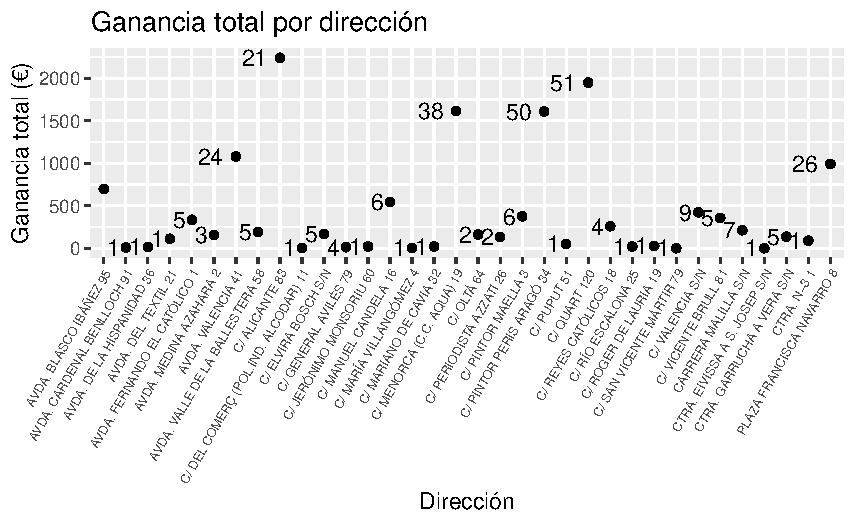
\includegraphics[width=0.9\linewidth]{ProyectoTD2025_files/figure-latex/grafica1-1}
En el gráfico anterior se puede observar que muchas direcciones cuentan
únicamente con una venta registrada. Sin embargo, hay dos supermercados
que destacan por tener un número de tickets significativamente superior
al resto. En general, se aprecia que a mayor número de tickets, mayor es
la ganancia total.

A continuación, comparamos las ganancias promedio por venta en cada
supermercado, para entender mejor su rendimiento individual más allá del
volumen total de ventas.

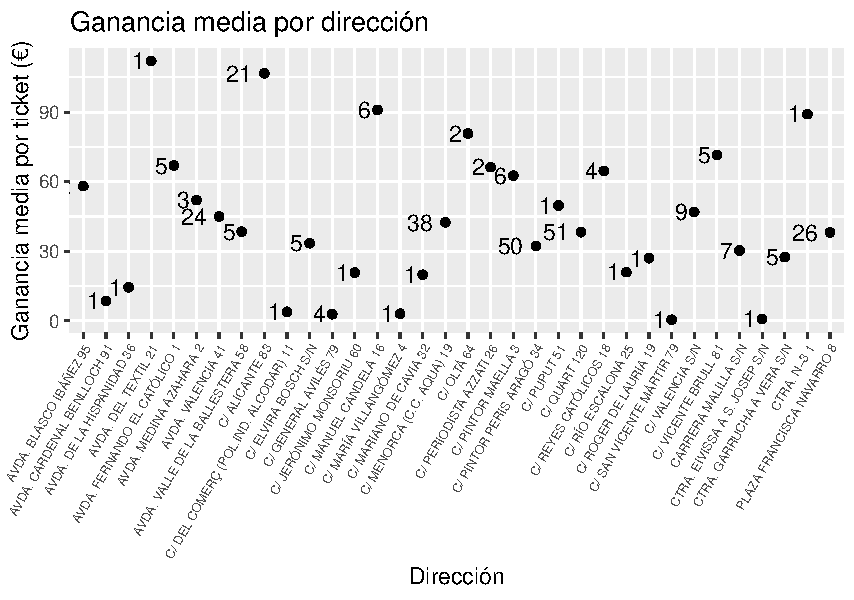
\includegraphics[width=0.9\linewidth]{ProyectoTD2025_files/figure-latex/grafica2-1}
En este segundo gráfico vemos que el supermercado ubicado en Calle
Alicante 83 sigue destacando en ingresos, aunque es el de Avenida del
Textil el que presenta una mayor ganancia media por ticket. Esto sugiere
un rendimiento más eficiente, a pesar de no tener el mayor volumen de
ventas.

\textbf{Relación entre el Número de Productos y el Precio Total por
Ticket}

En este apartado analizamos si existe una relación directa entre el
número de productos comprados en un ticket y el precio total pagado en
dicho ticket. Para ello, realizamos un gráfico de dispersión y
calculamos el coeficiente de correlación de Pearson.

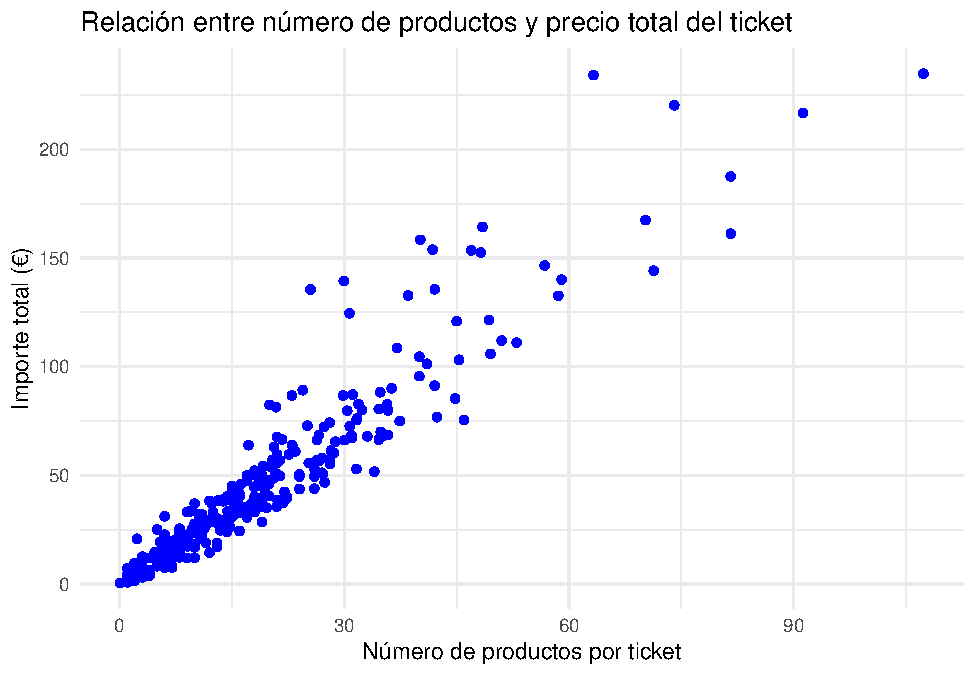
\includegraphics[width=0.85\linewidth]{ProyectoTD2025_files/figure-latex/grafica3-1}

El gráfico anterior muestra cómo varía el importe total del ticket en
función del número de productos adquiridos. Cada punto representa un
ticket diferente.

El coeficiente de correlación de Pearson es r cant\_precio, un valor
cercano a \(1\), lo cual indica que existe una relación lineal positiva
muy fuerte entre ambas variables. Es decir, cuantos más productos se
compran en un ticket, mayor es el importe total pagado, lo que resulta
coherente con el comportamiento esperado en compras de supermercado.

\bigskip

\hypertarget{preguntas}{%
\section{Preguntas}\label{preguntas}}

\hypertarget{cuuxe1les-son-los-5-productos-de-los-vendidos-por-unidades-con-muxe1s-ventas-cuuxe1ntas-unidades-de-cada-uno-se-han-vendido-y-por-kilos}{%
\subsection{- ¿Cuáles son los 5 productos, de los vendidos por unidades,
con más ventas ? ¿Cuántas unidades de cada uno se han vendido ? ¿Y por
kilos?}\label{cuuxe1les-son-los-5-productos-de-los-vendidos-por-unidades-con-muxe1s-ventas-cuuxe1ntas-unidades-de-cada-uno-se-han-vendido-y-por-kilos}}

\begin{longtable}[]{@{}llr@{}}
\caption{Top 5 productos más vendidos por unidades}\tabularnewline
\toprule\noalign{}
& nombre & cantidad \\
\midrule\noalign{}
\endfirsthead
\toprule\noalign{}
& nombre & cantidad \\
\midrule\noalign{}
\endhead
\bottomrule\noalign{}
\endlastfoot
110 & ATUN CLARO OLIVA & 62 \\
1083 & QUESO LONCHAS CABRA & 53 \\
164 & BOLSA PLASTICO & 51 \\
684 & LECHE DESNAT. CALCIO & 49 \\
1322 & YOGUR COCO & 40 \\
\end{longtable}

\begin{longtable}[]{@{}llr@{}}
\caption{Top 5 productos más vendidos por kilos}\tabularnewline
\toprule\noalign{}
& nombre & cantidad \\
\midrule\noalign{}
\endfirsthead
\toprule\noalign{}
& nombre & cantidad \\
\midrule\noalign{}
\endhead
\bottomrule\noalign{}
\endlastfoot
49 & PLATANO & 62.868 \\
5 & BANANA & 28.140 \\
56 & SANDIA BAJA SEMILLAS & 22.843 \\
42 & PEPINO & 19.624 \\
12 & CALABACIN VERDE & 17.754 \\
\end{longtable}

\hypertarget{si-consideramos-la-categoruxeda-de-frutas-y-verduras.-cuuxe1les-son-los-5-productos-muxe1s-vendidos-cuuxe1ntos-kilos-se-han-vendido-de-cada-uno-de-estos-productos}{%
\subsection{-Si consideramos la categoría de FRUTAS Y VERDURAS. Cuáles
son los 5 productos más vendidos ? ¿Cuántos kilos se han vendido de cada
uno de estos productos
?}\label{si-consideramos-la-categoruxeda-de-frutas-y-verduras.-cuuxe1les-son-los-5-productos-muxe1s-vendidos-cuuxe1ntos-kilos-se-han-vendido-de-cada-uno-de-estos-productos}}

\begin{longtable}[]{@{}llr@{}}
\caption{Top 5 productos más vendidos en la categoría Frutas y Verduras
(en kilos)}\tabularnewline
\toprule\noalign{}
& Producto & Kilos vendidos \\
\midrule\noalign{}
\endfirsthead
\toprule\noalign{}
& Producto & Kilos vendidos \\
\midrule\noalign{}
\endhead
\bottomrule\noalign{}
\endlastfoot
42 & PLATANO & 62.868 \\
5 & BANANA & 28.140 \\
49 & SANDIA BAJA SEMILLAS & 22.843 \\
35 & PEPINO & 19.624 \\
12 & CALABACIN VERDE & 17.754 \\
\end{longtable}

\hypertarget{si-consideramos-la-categoruxeda-de-pescado.-cuuxe1les-son-los-5-productos-muxe1s-vendidos-cuuxe1ntos-kilos-se-han-vendido-de-cada-uno-de-estos-productos}{%
\subsection{-Si consideramos la categoría de PESCADO. Cuáles son los 5
productos más vendidos ? ¿Cuántos kilos se han vendido de cada uno de
estos productos
?}\label{si-consideramos-la-categoruxeda-de-pescado.-cuuxe1les-son-los-5-productos-muxe1s-vendidos-cuuxe1ntos-kilos-se-han-vendido-de-cada-uno-de-estos-productos}}

\begin{longtable}[]{@{}llr@{}}
\caption{Top 5 productos más vendidos en la categoría Pescado (en
kilos)}\tabularnewline
\toprule\noalign{}
& Producto & Kilos vendidos \\
\midrule\noalign{}
\endfirsthead
\toprule\noalign{}
& Producto & Kilos vendidos \\
\midrule\noalign{}
\endhead
\bottomrule\noalign{}
\endlastfoot
1 & BACALADILLA & 3.180 \\
6 & DORADA & 2.934 \\
18 & SEPIA SUCIA REFRIG & 2.402 \\
17 & SEPIA LONJA & 2.000 \\
12 & RODABALLO & 1.788 \\
\end{longtable}

\hypertarget{muestra-mediante-un-gruxe1fico-de-luxedneas-como-ha-variado-el-precio-por-kilo-de-las-bananas-y-los-pluxe1tanos-en-los-tickets-disponibles-a-lo-largo-del-tiempo.}{%
\subsection{-Muestra mediante un gráfico de líneas como ha variado el
precio por kilo de las bananas y los plátanos en los tickets
disponibles, a lo largo del
tiempo.}\label{muestra-mediante-un-gruxe1fico-de-luxedneas-como-ha-variado-el-precio-por-kilo-de-las-bananas-y-los-pluxe1tanos-en-los-tickets-disponibles-a-lo-largo-del-tiempo.}}

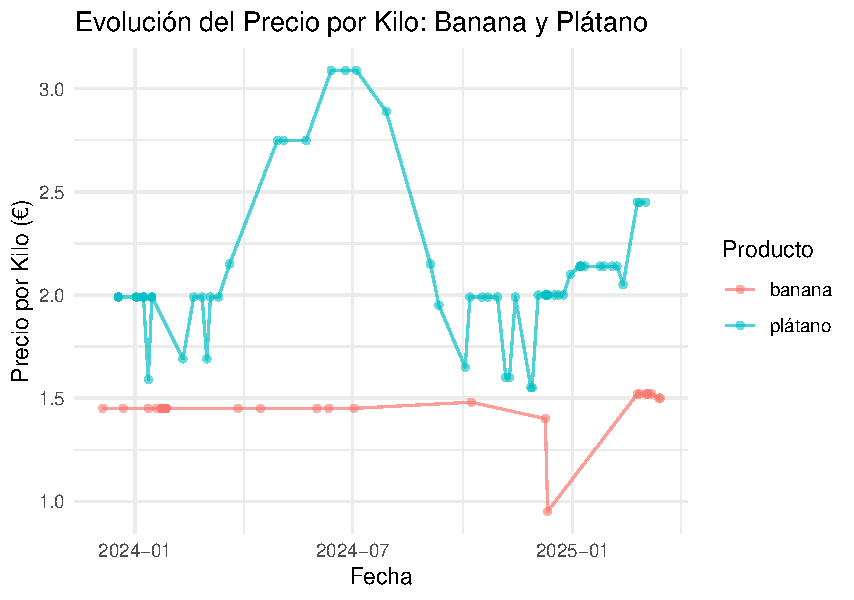
\includegraphics[width=0.9\linewidth]{ProyectoTD2025_files/figure-latex/unnamed-chunk-21-1}

\hypertarget{desde-quuxe9-ciudades-se-emiten-muxe1s-tickets}{%
\subsection{-¿Desde qué ciudades se emiten más
tickets?}\label{desde-quuxe9-ciudades-se-emiten-muxe1s-tickets}}

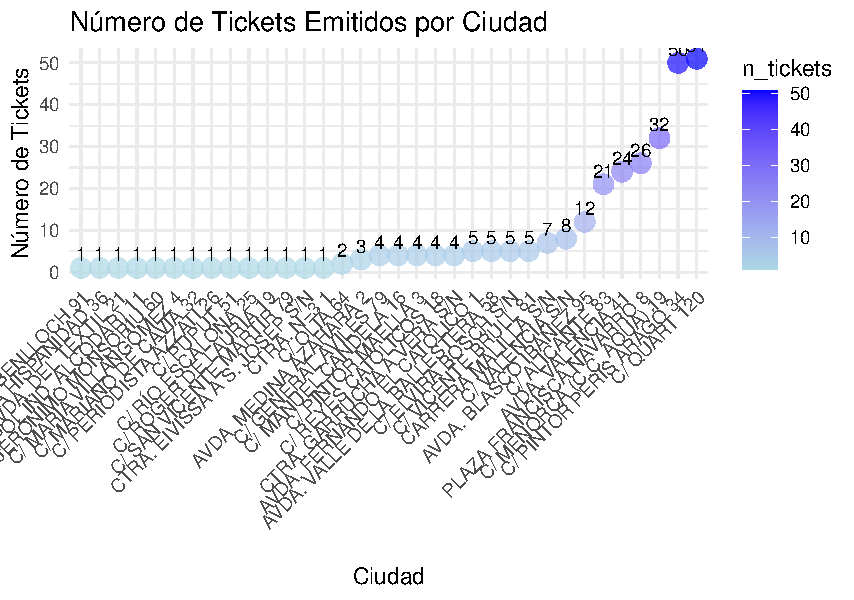
\includegraphics[width=0.9\linewidth]{ProyectoTD2025_files/figure-latex/unnamed-chunk-22-1}

La ciudad con más tickets emitidos es: C/ QUART 120Con un total de 51
tickets

\hypertarget{muestra-mediante-un-diagrama-el-nuxfamero-de-tickets-recogidos-cada-duxeda-de-las-semana.-si-tuvieses-que-cerrar-un-duxeda-entre-semana-quuxe9-duxeda-lo-haruxedas}{%
\subsection{-Muestra mediante un diagrama el número de tickets recogidos
cada día de las semana. ¿Si tuvieses que cerrar un día entre semana qué
día lo harías
?}\label{muestra-mediante-un-diagrama-el-nuxfamero-de-tickets-recogidos-cada-duxeda-de-las-semana.-si-tuvieses-que-cerrar-un-duxeda-entre-semana-quuxe9-duxeda-lo-haruxedas}}

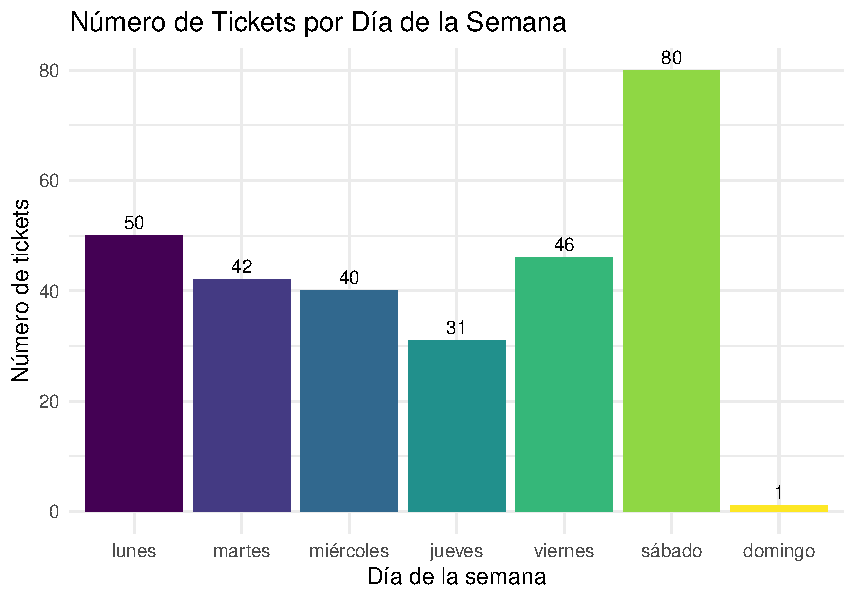
\includegraphics[width=0.9\linewidth]{ProyectoTD2025_files/figure-latex/unnamed-chunk-23-1}
Si se tubiera que cerrar un dia entre semana este seria el jueves que es
el dia que menos tickets se recogen.

\hypertarget{quuxe9-productos-han-generado-mayor-ingreso-total-precio-x-cantidad}{%
\subsection{-¿Qué productos han generado mayor ingreso total (precio x
cantidad)?}\label{quuxe9-productos-han-generado-mayor-ingreso-total-precio-x-cantidad}}

\begin{longtable}[]{@{}llr@{}}
\caption{Top 5 productos con mayor ingreso total}\tabularnewline
\toprule\noalign{}
& nombre & ingreso\_total \\
\midrule\noalign{}
\endfirsthead
\toprule\noalign{}
& nombre & ingreso\_total \\
\midrule\noalign{}
\endhead
\bottomrule\noalign{}
\endlastfoot
375 & alistado mediano & 31.3300 \\
3148 & bogavante crudo & 29.7000 \\
3853 & bacalao entero & 23.2034 \\
1842 & rodaballo & 19.7820 \\
4657 & salmon entero & 19.4068 \\
\end{longtable}

\hypertarget{cuuxe1l-es-el-ticket-con-el-mayor-importe-total-y-quuxe9-porcentaje-representa-este-ticket-respecto-al-importe-total-de-todos-los-tickets}{%
\subsection{-¿Cuál es el ticket con el mayor importe total y qué
porcentaje representa este ticket respecto al importe total de todos los
tickets?}\label{cuuxe1l-es-el-ticket-con-el-mayor-importe-total-y-quuxe9-porcentaje-representa-este-ticket-respecto-al-importe-total-de-todos-los-tickets}}

Respuesta: El ticket con el mayor importe total es el número 397921, con
un importe de 234,82 euros. Este ticket constituye el 1,67\% del importe
total de todos los tickets.

\par

\hypertarget{quuxe9-productos-se-compran-habitualmente-juntos-que-podemos-entender-sobre-la-dieta-de-los-clientes}{%
\subsection{-¿Qué productos se compran habitualmente juntos? ¿Que
podemos entender sobre la dieta de los
clientes?}\label{quuxe9-productos-se-compran-habitualmente-juntos-que-podemos-entender-sobre-la-dieta-de-los-clientes}}

\begin{longtable}[]{@{}llr@{}}
\caption{Los 10 productos que más se compran juntos}\tabularnewline
\toprule\noalign{}
item1 & item2 & frequency \\
\midrule\noalign{}
\endfirsthead
\toprule\noalign{}
item1 & item2 & frequency \\
\midrule\noalign{}
\endhead
\bottomrule\noalign{}
\endlastfoot
leche desnat. calcio & queso lonchas cabra & 44 \\
pan de pueblo & queso lonchas cabra & 43 \\
brotes tiernos maxi & queso lonchas cabra & 40 \\
plátano & queso lonchas cabra & 40 \\
queso fresco cabra & queso lonchas cabra & 40 \\
leche desn s/lact & queso lonchas cabra & 37 \\
act o\% nat ed 8 & queso lonchas cabra & 31 \\
filete pechuga & queso lonchas cabra & 30 \\
parking & queso lonchas cabra & 27 \\
queso lonchas cabra & zanahoria bolsa & 27 \\
\end{longtable}

Se han identificado pares de productos más frecuentemente comprados
juntos, donde uno de ellos es casi siempre QUESO LONCHAS CABRA. Eso
sugiere que este producto es muy popular y acompaña a muchos otros
productos a la misma compra.

\hypertarget{existen-diferencias-de-precios-para-el-mismo-producto-en-diferentes-tiendas-o-ubicaciones}{%
\subsection{-¿Existen diferencias de precios para el mismo producto en
diferentes tiendas o
ubicaciones?}\label{existen-diferencias-de-precios-para-el-mismo-producto-en-diferentes-tiendas-o-ubicaciones}}

\begin{longtable}[]{@{}llrr@{}}
\caption{Diferencias de precios para el mismo producto en diferentes
tiendas}\tabularnewline
\toprule\noalign{}
nombre & direccion & precio & n \\
\midrule\noalign{}
\endfirsthead
\toprule\noalign{}
nombre & direccion & precio & n \\
\midrule\noalign{}
\endhead
\bottomrule\noalign{}
\endlastfoot
+ proteína arandanos & AVDA. VALLE DE LA BALLESTERA 58 & 1.47 & 2 \\
+ proteína arandanos & PLAZA FRANCISCA NAVARRO 8 & 1.55 & 5 \\
+prot natilla choco & C/ ELVIRA BOSCH S/N & 1.75 & 4 \\
+prot natilla vaini & AVDA. BLASCO IBÁÑEZ 95 & 1.75 & 5 \\
+prot natilla vaini & AVDA. VALENCIA 41 & 1.75 & 1 \\
+prot pla-açaí & PLAZA FRANCISCA NAVARRO 8 & 1.15 & 2 \\
+proteínas café & C/ ELVIRA BOSCH S/N & 1.90 & 1 \\
1/2 conejo troceado & AVDA. VALENCIA 41 & 5.13 & 1 \\
1/2 conejo troceado & AVDA. VALENCIA 41 & 6.46 & 1 \\
1/2 conejo troceado & C/ ALICANTE 83 & 4.73 & 1 \\
\end{longtable}

\hypertarget{a-que-horas-del-dia-hay-muxe1s-ventas}{%
\subsection{-¿A que horas del dia hay más
ventas?}\label{a-que-horas-del-dia-hay-muxe1s-ventas}}

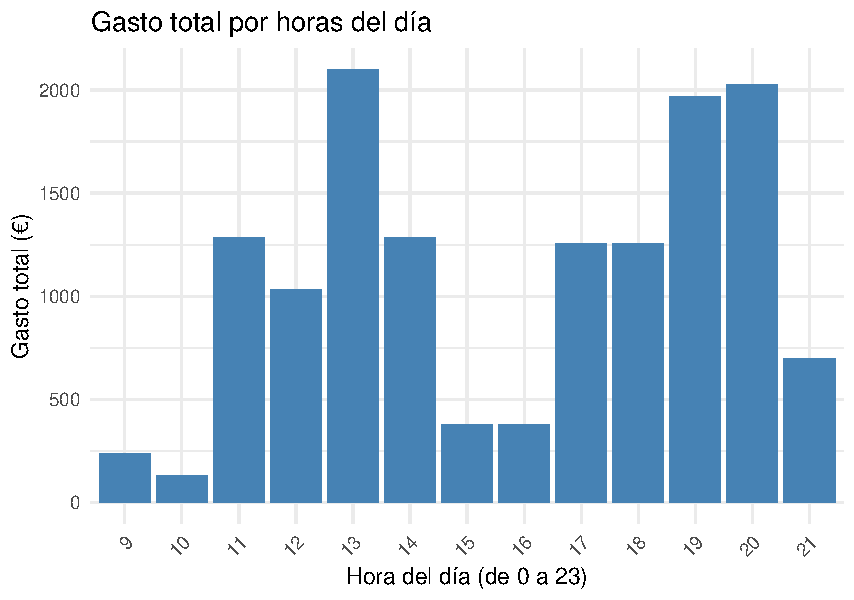
\includegraphics[width=0.9\linewidth]{ProyectoTD2025_files/figure-latex/unnamed-chunk-28-1}

\hypertarget{en-cuantos-tickets-se-venden-frutasverduras-y-pescados}{%
\subsection{-En cuantos tickets se venden frutas/verduras y
pescados?}\label{en-cuantos-tickets-se-venden-frutasverduras-y-pescados}}

Número de tickets en los que se venden frutas/verduras: 168 Número de
tickets en los que se venden pescados: 24

\hypertarget{existen-diferencias-de-consumo-por-cada-mercadona}{%
\subsection{-¿Existen diferencias de consumo por cada
mercadona?}\label{existen-diferencias-de-consumo-por-cada-mercadona}}

\begin{longtable}[]{@{}
  >{\raggedright\arraybackslash}p{(\columnwidth - 6\tabcolsep) * \real{0.4932}}
  >{\raggedleft\arraybackslash}p{(\columnwidth - 6\tabcolsep) * \real{0.1644}}
  >{\raggedleft\arraybackslash}p{(\columnwidth - 6\tabcolsep) * \real{0.1918}}
  >{\raggedleft\arraybackslash}p{(\columnwidth - 6\tabcolsep) * \real{0.1507}}@{}}
\caption{Estadísticas de Gasto Promedio, Mediana y Desviación Estándar
por Mercadona}\tabularnewline
\toprule\noalign{}
\begin{minipage}[b]{\linewidth}\raggedright
direccion
\end{minipage} & \begin{minipage}[b]{\linewidth}\raggedleft
media\_gasto
\end{minipage} & \begin{minipage}[b]{\linewidth}\raggedleft
mediana\_gasto
\end{minipage} & \begin{minipage}[b]{\linewidth}\raggedleft
desv\_gasto
\end{minipage} \\
\midrule\noalign{}
\endfirsthead
\toprule\noalign{}
\begin{minipage}[b]{\linewidth}\raggedright
direccion
\end{minipage} & \begin{minipage}[b]{\linewidth}\raggedleft
media\_gasto
\end{minipage} & \begin{minipage}[b]{\linewidth}\raggedleft
mediana\_gasto
\end{minipage} & \begin{minipage}[b]{\linewidth}\raggedleft
desv\_gasto
\end{minipage} \\
\midrule\noalign{}
\endhead
\bottomrule\noalign{}
\endlastfoot
AVDA. DEL TEXTIL 21 & 112.02000 & 112.020 & NA \\
C/ ALICANTE 83 & 106.74905 & 132.730 & 70.4205855 \\
C/ MANUEL CANDELA 16 & 90.96500 & 96.780 & 42.6520779 \\
CTRA. N-3 1 & 89.18000 & 89.180 & NA \\
C/ OLTÁ 64 & 80.78000 & 80.780 & 89.6469977 \\
C/ VICENTE BRULL 81 & 71.45800 & 55.220 & 70.8771580 \\
AVDA. FERNANDO EL CATÓLICO 1 & 66.98800 & 57.330 & 25.5122455 \\
C/ PERIODISTA AZZATI 26 & 66.30000 & 66.300 & 0.0000000 \\
C/ REYES CATÓLICOS 18 & 64.68750 & 62.350 & 48.3358089 \\
C/ PINTOR MAELLA 3 & 62.62000 & 62.710 & 42.3117586 \\
AVDA. BLASCO IBÁÑEZ 95 & 58.12167 & 60.845 & 28.5231794 \\
AVDA. MEDINA AZAHARA 2 & 52.07333 & 52.120 & 0.8609491 \\
C/ PUPUT 51 & 49.74000 & 49.740 & NA \\
C/ VALENCIA S/N & 46.94000 & 45.610 & 21.3230128 \\
AVDA. VALENCIA 41 & 45.02083 & 32.490 & 36.0782802 \\
C/ MENORCA (C.C. AQUA) 19 & 42.47974 & 36.715 & 26.4792739 \\
AVDA. VALLE DE LA BALLESTERA 58 & 38.45400 & 38.620 & 24.2723975 \\
C/ QUART 120 & 38.23176 & 37.000 & 18.6523093 \\
PLAZA FRANCISCA NAVARRO 8 & 38.15846 & 35.515 & 17.5759747 \\
C/ ELVIRA BOSCH S/N & 33.48200 & 30.940 & 16.0079221 \\
C/ PINTOR PERIS ARAGÓ 34 & 32.19840 & 24.200 & 23.8732468 \\
CARRERA MALILLA S/N & 30.32571 & 25.500 & 16.0475209 \\
CTRA. GARRUCHA A VERA S/N & 27.46600 & 31.370 & 11.6894388 \\
C/ ROGER DE LAURIA 19 & 26.98000 & 26.980 & NA \\
C/ RÍO ESCALONA 25 & 20.99000 & 20.990 & NA \\
C/ JERÓNIMO MONSORIU 60 & 20.80000 & 20.800 & NA \\
C/ MARIANO DE CAVIA 32 & 19.85000 & 19.850 & NA \\
AVDA. DE LA HISPANIDAD 36 & 14.46000 & 14.460 & NA \\
AVDA. CARDENAL BENLLOCH 91 & 8.50000 & 8.500 & NA \\
C/ DEL COMERÇ (POL.IND. ALCODAR) 11 & 3.90000 & 3.900 & NA \\
C/ MARÍA VILLANGÓMEZ 4 & 3.08000 & 3.080 & NA \\
C/ GENERAL AVILÉS 79 & 2.85000 & 2.500 & 1.4525839 \\
CTRA. EIVISSA A S. JOSEP S/N & 0.77000 & 0.770 & NA \\
C/ SAN VICENTE MÁRTIR 79 & 0.43000 & 0.430 & NA \\
\end{longtable}

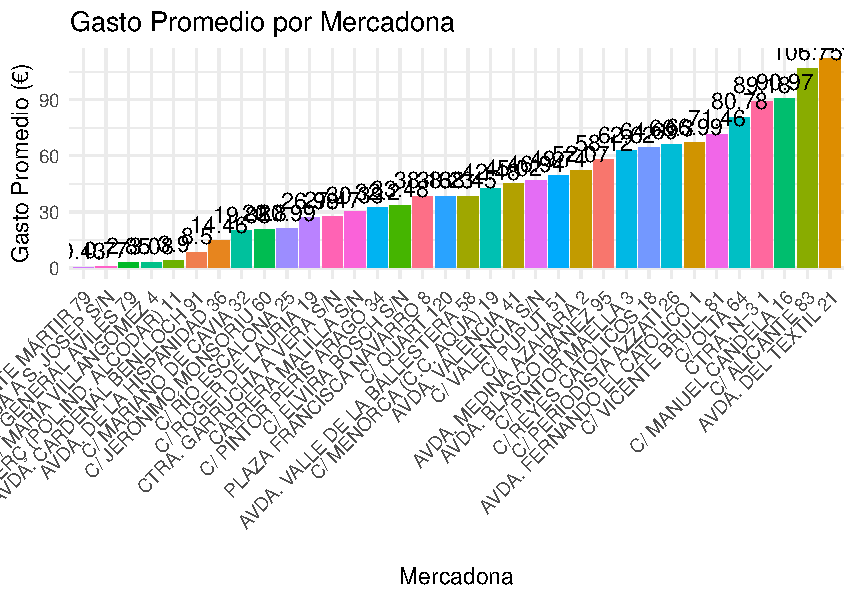
\includegraphics[width=0.9\linewidth]{ProyectoTD2025_files/figure-latex/unnamed-chunk-30-1}

\hypertarget{que-mes-y-que-dia-del-auxf1o-es-cuando-mas-dinero-se-gasta}{%
\subsection{-¿Que mes y que dia del año es cuando mas dinero se
gasta?}\label{que-mes-y-que-dia-del-auxf1o-es-cuando-mas-dinero-se-gasta}}

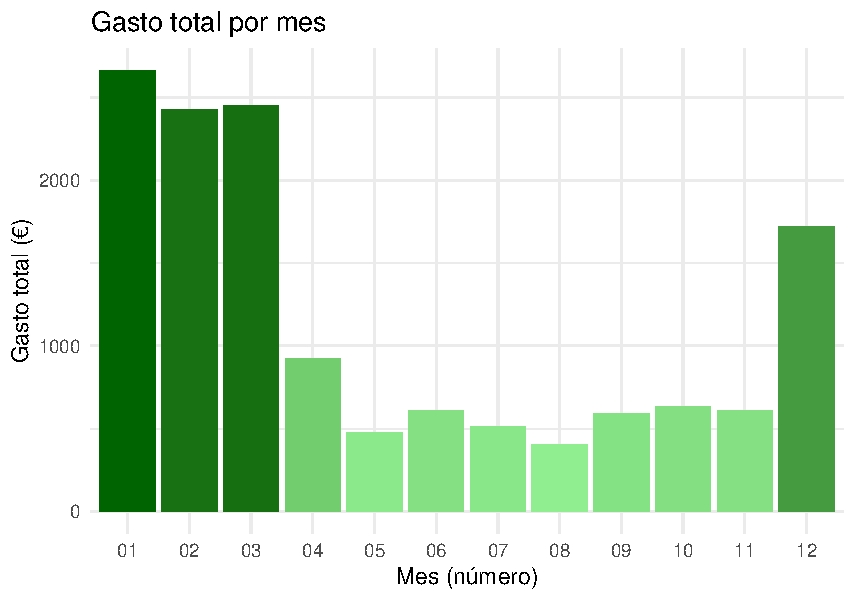
\includegraphics[width=0.9\linewidth]{ProyectoTD2025_files/figure-latex/unnamed-chunk-31-1}

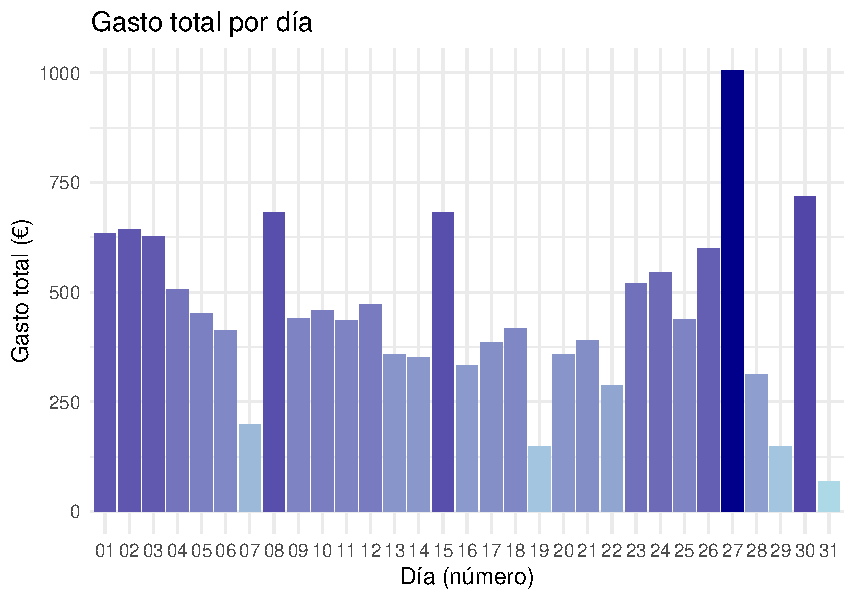
\includegraphics[width=0.9\linewidth]{ProyectoTD2025_files/figure-latex/unnamed-chunk-32-1}
El mes con más gasto es el mes 01 con un total de 2663.99€. El día con
más gasto es el día 27 con un total de 1005.7€.

\hypertarget{cuuxe1l-es-las-categoruxeda-de-productos-con-mayor-venta-en-tuxe9rminos-de-cantidad-y-cuuxe1l-es-su-contribuciuxf3n-porcentual-al-total-de-unidades-vendidas-hay-relaciuxf3n-entre-otras-categoruxedas}{%
\subsection{-¿Cuál es las categoría de productos con mayor venta en
términos de cantidad, y cuál es su contribución porcentual al total de
unidades vendidas? Hay relación entre otras
categorías?}\label{cuuxe1l-es-las-categoruxeda-de-productos-con-mayor-venta-en-tuxe9rminos-de-cantidad-y-cuuxe1l-es-su-contribuciuxf3n-porcentual-al-total-de-unidades-vendidas-hay-relaciuxf3n-entre-otras-categoruxedas}}

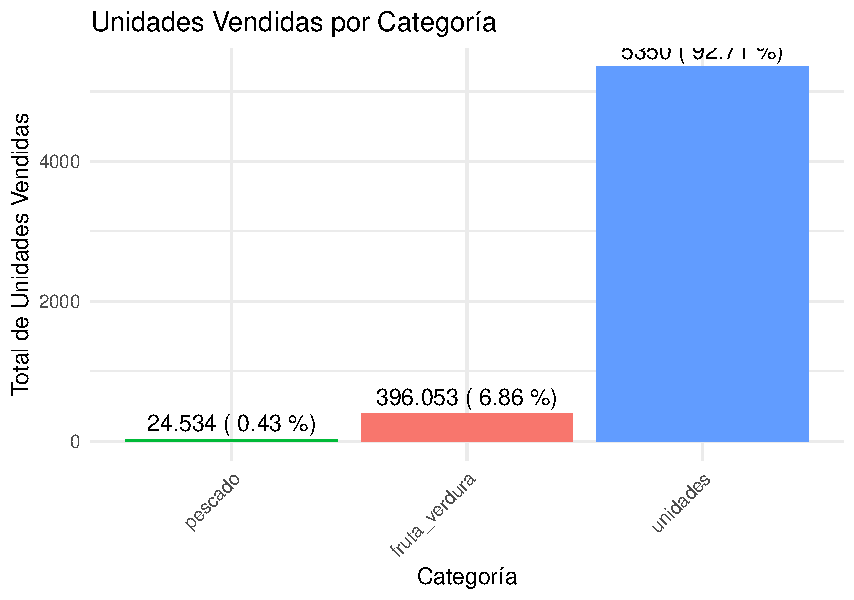
\includegraphics[width=0.9\linewidth]{ProyectoTD2025_files/figure-latex/unnamed-chunk-33-1}

\hypertarget{conclusiones}{%
\section{Conclusiones}\label{conclusiones}}

A través del análisis detallado de los tickets de compra, se han
obtenido importantes hallazgos sobre los patrones de consumo en los
distintos establecimientos. Hemos identificado qué productos son los más
y menos vendidos, tanto por unidades como por kilos, así como aquellos
que generan mayor ingreso. También se han detectado diferencias de
precios del mismo producto entre tiendas, lo que podría deberse a
políticas de precios locales o promociones específicas.

El estudio de los tickets ha permitido observar variaciones en el
comportamiento de compra a lo largo de la semana, el mes y el día,
identificando los momentos de mayor y menor actividad. Esto puede ser
útil para tomar decisiones operativas, como optimizar horarios de
apertura o reforzar personal en momentos clave. Además, se han detectado
combinaciones frecuentes de productos, lo que aporta pistas sobre los
hábitos alimenticios de los clientes, reflejando un patrón de consumo
alineado con una dieta mediterránea basada en frutas, verduras y
pescado.

En conjunto, estos análisis ofrecen una base sólida para tomar
decisiones estratégicas orientadas a mejorar la eficiencia, ajustar la
oferta de productos y potenciar la rentabilidad de cada tienda.

%%%%%%%%%%%%%%%%%%%%%%%%%%%%%%%%%%%%%%%%%%

\vspace{6pt}

%%%%%%%%%%%%%%%%%%%%%%%%%%%%%%%%%%%%%%%%%%
%% optional

% Only for the journal Methods and Protocols:
% If you wish to submit a video article, please do so with any other supplementary material.
% \supplementary{The following supporting information can be downloaded at: \linksupplementary{s1}, Figure S1: title; Table S1: title; Video S1: title. A supporting video article is available at doi: link.}

%%%%%%%%%%%%%%%%%%%%%%%%%%%%%%%%%%%%%%%%%%







%%%%%%%%%%%%%%%%%%%%%%%%%%%%%%%%%%%%%%%%%%
%% Optional

%% Only for journal Encyclopedia


%%%%%%%%%%%%%%%%%%%%%%%%%%%%%%%%%%%%%%%%%%
%% Optional
%%%%%%%%%%%%%%%%%%%%%%%%%%%%%%%%%%%%%%%%%%
\begin{adjustwidth}{-\extralength}{0cm}

%\printendnotes[custom] % Un-comment to print a list of endnotes



% If authors have biography, please use the format below
%\section*{Short Biography of Authors}
%\bio
%{\raisebox{-0.35cm}{\includegraphics[width=3.5cm,height=5.3cm,clip,keepaspectratio]{Definitions/author1.pdf}}}
%{\textbf{Firstname Lastname} Biography of first author}
%
%\bio
%{\raisebox{-0.35cm}{\includegraphics[width=3.5cm,height=5.3cm,clip,keepaspectratio]{Definitions/author2.jpg}}}
%{\textbf{Firstname Lastname} Biography of second author}

%%%%%%%%%%%%%%%%%%%%%%%%%%%%%%%%%%%%%%%%%%
%% for journal Sci
%\reviewreports{\\
%Reviewer 1 comments and authors’ response\\
%Reviewer 2 comments and authors’ response\\
%Reviewer 3 comments and authors’ response
%}
%%%%%%%%%%%%%%%%%%%%%%%%%%%%%%%%%%%%%%%%%%
\PublishersNote{}
\end{adjustwidth}


\end{document}
